\documentclass[a4paper]{article}

\usepackage[english]{babel}
\usepackage[utf8x]{inputenc}
\usepackage{amsmath}
\usepackage{amssymb}
\usepackage{float}
\usepackage{graphicx}
\usepackage[colorinlistoftodos]{todonotes}
\usepackage[authoryear]{natbib}
\usepackage{hyperref}
\usepackage{authblk}
\usepackage[margin=1in]{geometry}
\usepackage{pgfplots}
\pgfplotsset{compat=1.12}
\usepackage{biblatex} %Imports biblatex package
\addbibresource{Bibliography.bib} %Import the bibliography file

\usepackage[inline,ignoremode]{trackchanges} % Documentation of this package can be found at http://trackchanges.sourceforge.net/
\addeditor{MWS} % For each editor, repeat this command with their initials. Monroe is added by default.


\title{\vspace{-1cm}COVID-19 Prediction from Symptoms}
\author{Guankai Zhai, Weiyan Wu, Jianyang Zhou}
\date{\today} % You can write in any date within the brackets.

\begin{document}

\maketitle

\begin{abstract}
We cleaned our data set and conducted some exploratory data analysis (EDA) to determine which symptoms are highly linked to a positive diagnosis of COVID-19. We fitted several classification models on this dataset and compared their performance metrics with different hyperparameters. We also proposed future work that is planned for the second half of the semester. 
\end{abstract}
\section*{Introduction}
As the world began to mount an unprecedented worldwide response to COVID- 19 in early 2020, it lacked a standardized, global way to measure COVID-19 illness and track the pandemic that would help guide decision-making (e.g., implementation of social distancing measures). Thus, a model to identify infected patients from the symptoms they display is urgently needed. \par
The Israeli Ministry of Health publicly released data of all
individuals who were tested for SARS-CoV-2 via RT-PCR assay of a
nasopharyngeal swab \cite{data}. We leveraged this data to build a classifier which, given a patient's indicated symptoms, could classify the patient as either being infected or not.


\section*{Data Cleaning and Preparation}
We first imported the dataset into a Jupyter Notebook. The dataset contains 765,1053 observations each with 10 dimensions. With one dimension being the date of the test, 8(cough, fever, sore throat, breath shortness, headache, age 60 and above, gender, and test result) of the remaining 9 dimensions are binary variables and 1(test indication) has three categories. \par
We then drop observations that are corrupt (i.e contain NaN values). After this, we are left with 597,7416 entries. With some of the data being in Hebrew, we used GoogleTrans to translate these entries into English for better interpretability. We also changed categorical variables with string representations into 0s and 1s. \par
Finally, we used one-hot encoding to encode the dimension of "test indication", which could be "Contact traced," "Abroad," or "Other."

\section*{Exploratory Data Analysis}
We then began to conduct some exploratory analysis on our data to determine what is relevant with the test result.
We start by plotting the number of positive cases over time. \par
\begin{figure}[H]
\centering
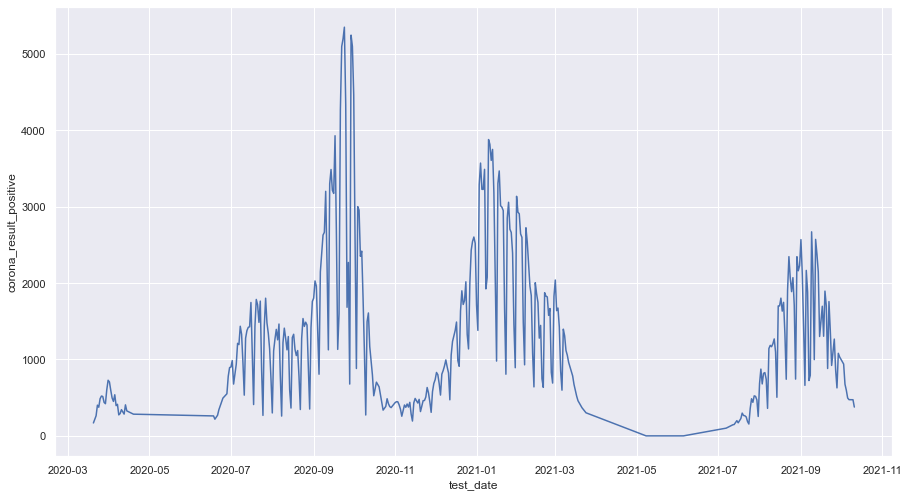
\includegraphics[scale=0.265]{total.png}
\caption{Total Number of Positive Cases with Time.}
\label{Confirmed Cases}
\end{figure}
We find that the number of positive cases vary with time and that the pandemic comes in the form of waves: the number of total positive cases would increase up until a certain point, after which it started to go down. This cycle has repeated several times since the onset of this pandemic. Thus, we believe that warnings about upcoming waves are essential for policy making and supply chain preparations, which will be discussed in greater details in the last section of this report. \par
We then start exploring factors that change the probability of the tests being positive. Intuitively, the patient having any of the listed symptoms would mean that his/her test is more likely to be positive. We summarize the statistical results below.\par
\begin{table}[H]
\centering
\caption{Proportion of Positive Tests Given a Symptom}
\begin{tabular}{| l | c | c | c | c | c |}
\hline
Symptom & Cough & Fever & Sore Throat & Shortness of Breath & Headache  \\ \hline
w/o Symptom & 7.2 & 7.3 & 7.9 & 8.4 & 7.2 \\ \hline
w/ Symptom & 37.9 & 41.8 & 43.0 & 51.2 & 43.5 \\
\hline
\end{tabular}
\label{Table}
\end{table}

We then start to explore the relationship between the proportion of positive cases and the other characteristics, which is even more interesting. We tabulate our results below, in a similar fashion to the last part.
\begin{table}[H]
\centering
\caption{Proportion of Positive Tests Given a Characteristic}
\begin{tabular}{| l | c | c | c | c |}
\hline
Characteristic & Being Male & $Age \ge 60$ & Being Abroad & Contact Traced  \\ \hline
w/o Characteristic & 8.8 & 8.7 & 8.6 & 5.4 \\ \hline
w/ Characteristic & 8.3 & 8.1 & 11.2 & 43.9 \\
\hline
\end{tabular}
\label{Table}
\end{table}

\section*{Models}
Given the above exploratory analysis, we can conclude that all symptoms in the dataset as well as some characteristics(Being Abroad and Contact Traced) have an impact on the chance that a test is positive. We thus include these as our features. We did not include all possible features to prevent overfitting. We choose the test results (either 1 or 0) as our labels. We then separated our data into training and testing datasets. Since the original dataset is large, we only used $0.5\%$ of our data for validation, which is more than 5000 observations and should give us a very accurate estimate of our models' performance according to the Central Limit Theorem. \par
To evaluate the performance of our models, we will look at the overall k-cross-validated accuracy as well as the false-positive and false-negative rates. Since testing a patient is not particularly expensive but missing an infected patient has a large negative externality, we prefer a small false negative rate and are willing to accept a relatively high false positive rate. \par
Since we excluded features are shown to have little impact on the positive rate and our sample size is relatively large, we believe that overfitting is not very likely.

\subsection*{Logistic Regression}
We first built a classifier with Logistic Regression. The reason we used this as our first model was that logistic regression could produce the probabilities of each label, which is very helpful if we want to control our false positive/negative rate. However, the accuracy of this model, at $76\%$ after cross validation, is not particularly impressive.\par
However, if we decrease our threshold of positive to 0.2 (i.e. any patient whose probability of being positive is greater than 0.3 will be classified as positive), our false negative rate will decrease to 0.15, which is satisfactory. As the following diagram shows, an even lower false negative rate (FNR) could be achieved at the expense of a higher false positive rate(FPS).\par
\begin{figure}[H]
\centering
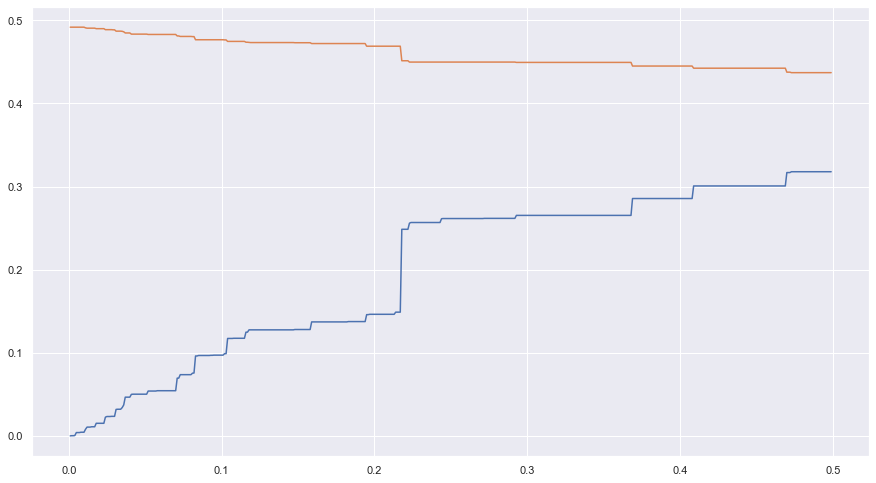
\includegraphics[scale=0.265]{fps.png}
\caption{FPR(Orange) and FNR(Blue) with Decision Threshold.}
\label{COnfirmed Cases}
\end{figure}

\subsection*{K-Nearest Neighbors}
We then try to build our classifier with the k-Nearest Neighbors Algorithm. The central assumption here is that patients with similar features would have the same label. This is a reasonable assumption to make in our case.\par
k-NN has an important hyperparameter: the number of neighbors that we will look at. We tuned this parameter with a for-loop. The accuracy of each k value is presented in the following graph.
\begin{figure}[H]
\centering
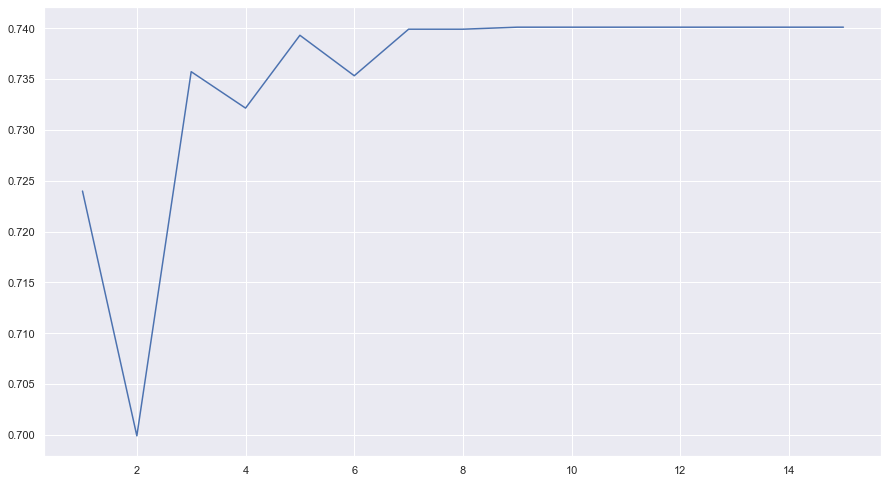
\includegraphics[scale=0.265]{knn.png}
\caption{Accuracy of kNN with Different Values of k.}
\label{COnfirmed Cases}
\end{figure}
As it could be seen, the performance of our kNN algorithm is not that better compared to the above logistic regression. However, the running time of this model was significantly higher than logistic regression during tests, despite having a shorter training time. Thus, this model is inappropriate for our situation in which we will run the fitted model many times for many patients.

\section*{Future Work}
Given the limited time available for this part of the project, some work remains to be done. This includes but is not limited to the following points.
\begin{itemize}
  \item Further analyses on more models for the above prediction challenge. Several possiblities include trees and random forests,  support vector machines, etc. Discussions on the recall and precision rates could also be added.
  \item A warning system should be built to give alerts about upcoming waves of the pandemic in advance. To achieve this, we plan on integrating the dataset of the daily number of confirmed COVID cases in Israel into our current data. We will then build a regression model to predict the number of cases that will be confirmed in the coming week based on information of the past week.
  \item A major limitation currently is that COVID-19 patients display very similar symptoms to influenza patients, making prediction difficult. We thus plan to build a Deep Neural Network (with its final layer using the softmax function as activation) to classify patients as either having COVID-19, influenza, or neither. This also requires us to collect an additional dataset that contains this information.
\end{itemize}

\printbibliography


\end{document}

